The equal-call controls separate natural-language convention from executable decision visibility (Figure~\ref{fig:submission-critical-effects}). Convention-told effects are model-conditional (Qwen -5.0, GLM +10.0, DeepSeek +7.5, MiniMax +25.0 pp), whereas Decision-visible improves changed PairAcc for all four models (Qwen +25.0, GLM +53.1, DeepSeek +43.8, MiniMax +34.4 pp). The panels use different frozen inventories and are not pooled; Convention and decision-block runs contain 1 and 0 incomplete ITT rows, respectively.

\begin{figure}[t]
\centering
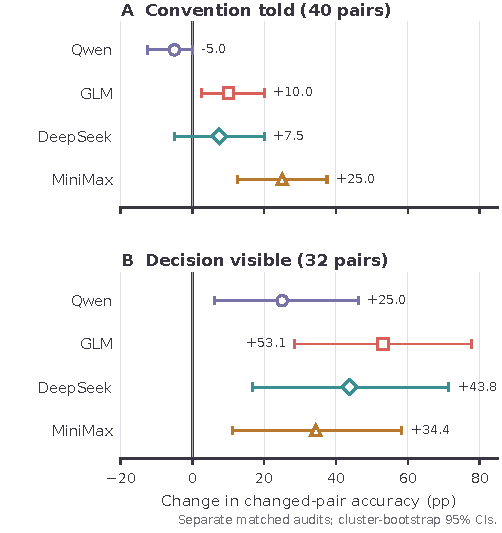
\includegraphics[width=0.97\columnwidth]{Figures/fig_submission_critical_pairacc_effects.pdf}
\caption{Post-primary equal-call contrasts. A: natural-language convention only (40 changed pairs). B: complete decision block visible to the actor (32 actionable changed pairs). Bars are cluster-bootstrap 95\% CIs; inventories are separate and unpooled.}
\label{fig:submission-critical-effects}
\end{figure}
